\documentclass[]{article}

\usepackage[utf8]{inputenc}
\usepackage[paperheight=0.6in,paperwidth=1in,margin=.1mm]{geometry}
\usepackage{tikz}
\usetikzlibrary{shapes, arrows, calc}
\usepackage{color}

\usepackage{booktabs}  % nicer table borders 

\begin{document}

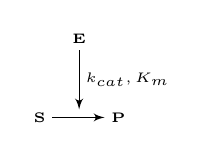
\begin{tikzpicture}[>=latex']
\tiny
\node  at (0, 0)  (S) {$\bf S$};
\node  at (.5, 1) (E) {$\bf E$};
\node  at (1, 0)  (P) {$\bf P$};
\path (S) edge[->] (P);
\path (E) edge[->] node[right] {$k_{cat}, K_m$} ($(S)!0.5!(P)+(0, 0.1)$);
\end{tikzpicture} 
\end{document}

